\documentclass{TUBAFarbeiten}
\usepackage[T1]{fontenc}
\usepackage[singlespacing]{setspace}
\usepackage{hyperref}
\usepackage{graphics}
\usepackage{wrapfig}
\usepackage{listings}
\usepackage{xcolor}
\usepackage{float}

%\usepackage{TUBAFbib}
%\usepackage[zitatstil=chron,autor=textsc]{TUBAFbib}
\usepackage[utf8]{inputenc}
\usepackage[nottoc,numbib]{tocbibind}



\lstdefinestyle{customc}{
  belowcaptionskip=1\baselineskip,
  breaklines=true,
  frame=L,
  xleftmargin=\parindent,
  language=C,
  showstringspaces=false,
  basicstyle=\footnotesize\ttfamily,
  keywordstyle=\bfseries\color{green!40!black},
  commentstyle=\itshape\color{purple!40!black},
  identifierstyle=\color{blue},
  stringstyle=\color{orange},
}

\TUBAFFakultaet{Fakultät für Mathematik und Informatik}
\TUBAFInstitut{Institut für Informatik}

\TUBAFTitel{Exploring Data Structures in C: Deque}
\TUBAFAutor[M. Naumann]{Marco Naumann}
\TUBAFStudiengang{Angewandte Informatik}
\TUBAFMatrikel{64645}
\TUBAFDatum[2021 09 18]{15.09.2021}

\begin{document}


\maketitle
\tableofcontents
\newpage
\section{Einleitung}
Mit zunehmender Komplexität von Programmen und Programmieraufgaben in allen Bereichen der Softwareentwicklung stößt man schnell an die Grenzen konventioneller Datenstrukturen, wie Arrays, etc. Um die Funktionalitäten dieser zu erweitern, müssen neue, komplexere, Datenstrukturen implementiert werden, wie z.B. \textit{Trie}, \textit{Heap}, \textit{Hashmap}. 
\newline Ein weiteres Beispiel für eine komplexere Datenstruktur wäre die Double-Ended-Queue (kurz. Deque), welche einen schnellen Zugriff auf das älteste eingefügte Element und das neuste eingefügte Element einer Objektmenge bietet und so z.B. Anwendung in Work-Stealing-Algorithmen findet.
Im Folgendem wird der Aufbau und mögliche Implementierung dieser Datenstruktur in C dargelegt. Der Vorteil der Deque, welcher in den schnellen Zugriffszeiten der oben beschriebenen Stellen besteht, wird anhand einiger Beispiele gezeigt.    

\section{Grundlagen}
In Anbetracht dessen, dass die Double-Ended-Queue eine Unterform der Queue ist, wird im Folgenden zu Beginn die Datenstruktur Queue kurz erklärt.\newline
In der Informatik wird die klassische Warteschlange als eine sequenzielle Ansammlung von Objekten dargestellt. Diese Objektsammlung kann man verändern, indem man weitere Daten von einer Seite anhängt oder der anderen entfernt. 
Durch Betrachtung von Warteschlangen wie man diese in der Realität vorfindet und wie sie von Menschen geformt wird, wurde folgende Konvention gefasst: Das Ende, an welchem Objekte angehängt werden, wird als \textit{Back} oder \textit{Tail} bezeichnet und das Ende, an welchem diese entfernt werden, als \textit{Head} oder \textit{Front}. 
Aufgrund dessen, dass man bei einer klassischen Warteschlange nur Objekte an einer Seite einfügt und an einer anderen entfernt, identifiziert man diese als eine FIFO\footnote{„First In – First Out, ist gleichbedeutend mit „First come, first served” und bezeichnet jegliche das Verfahren der Speicherung, bei denen diejenigen Elemente, die zuerst gespeichert wurden, auch zuerst wieder aus dem Speicher entnommen werden.“ - \url{https://de.wikipedia.org/wiki/First_In_-_First_Out}} Datenstruktur.
Der Zugriff auf einzelne Objekte in der Warteschlange ist somit abhängig vom Objekt, auf welches zugegriffen werden soll. Soll auf das Head-Objekt zugegriffen werden, ist dieses direkt verfügbar und mit O(1) Iterationsschritten abrufbar. Nach dem Abruf des alten Head-Objekts kann nun auf das dahinter befindliche wieder mit O(1) zugegriffen werden, da dies nun das Head-Objekt ist. Betrachtet man jedoch individuelle Objekte, werden O(n) Iterationen benötigt, um ein beliebiges Objekt mit einer Warteschlange von der Länge n zur Verfügung zu stellen. Somit wird zuerst durch die ganze Datenstruktur iteriert, wenn auf das Tail-Objekt zugegriffen werden soll. Dies kann bei langen Warteschlangen, mitunter vergleichbar viel Zeit in Anspruch nehmen.\newline
Daher der Grundgedanke der Deque. Im Gegensatz zur Queue kann die Deque sowohl am Head als auch am Tail Objekte entgegen nehmen und diese wieder ausgeben, was den Hauptunterschied zur klassischen Warteschlange darstellt \cite[238]{maclaren1969art}. Somit liefert die Deque in der Standard-Implementierung  sowohl für den Head als auch den Tail dieselben Funktionen, welche bei der normalen Warteschlange nur einmalig existieren. So hat der Head eine Push-Funktion, welche Daten der Warteschlange anhängt, aber auch der Tail bietet diese Funktionalitäten. Genauso haben beide eine Pop-Funktion, welche eben diese der Warteschlange wieder entnimmt. Optional und häufig bei umfangreicheren Implementierungen zu finden ist eine Peek-Funktion, welche es ermöglicht die Daten am Head, oder Tail abzurufen ohne diese der Warteschlange zu entfernen. Durch eine derartige Implementierung ist für den Head und Tail eine Zugriffsgeschwindigkeit von O(1) gewährleistet, wodurch die Datenstruktur jedoch an Komplexität zunimmt. Hierbei zu beachten gilt, dass eine Deque nicht fundamental besser als die klassische Warteschlange ist, jedoch in spezifischen Anwendungen andere Datenstrukturmodelle an Performance übertrifft. Eines der besten Beispiele, wofür eine Deque verwendet werden kann, ist ein Work-Stealing-Algorithm worauf im späteren Verlauf unter \ref{WorkStealing} genauer eingegangen wird.
\section{Aufbau der Deque}
Um in der Lage zu sein, einen sofortigen Zugriff auf das Head-, bzw. Tail-Objekt in der Datenstruktur zu ermöglichen, müssen beide Positionen bekannt sein. Durch Pointer auf das entsprechende Head-, oder Tail-Objekt ist es möglich, die Speicheradresse eben dieser zu speichern, was einen direkten Abruf der Daten zu einem späteren Zeitpunkt ermöglicht. Nach einem Zugriff müssen die gespeicherten Adressen der Pointer lediglich wieder auf den neuen Head oder Tail angepasst werden, um einen wiederholten Abruf dieser zu ermöglichen. Umgekehrt erfolgt dies beim Versuch ein Objekt in die Datenstruktur zu speichern. Hierbei muss beim Versuch, Daten in die Deque zu legen, der Head-, bzw. Tail-Pointer auf eine neue, zu dem Zeitpunkt undefinierte bzw. leere, Speicherzelle versetzt werden und im Anschluss daran die Daten dorthinein gespeichert werden. Nun gibt es historisch verschiedene Möglichkeiten, Daten zu speichern, und diese zu organisieren, somit gibt es verschiedene Möglichkeiten eine Deque zu implementieren \cite[2]{horowitz1976fundamentals}.
\subsection{Deque mit Fixierter Länge}
\begin{wrapfigure}{l}{0.4\textwidth}
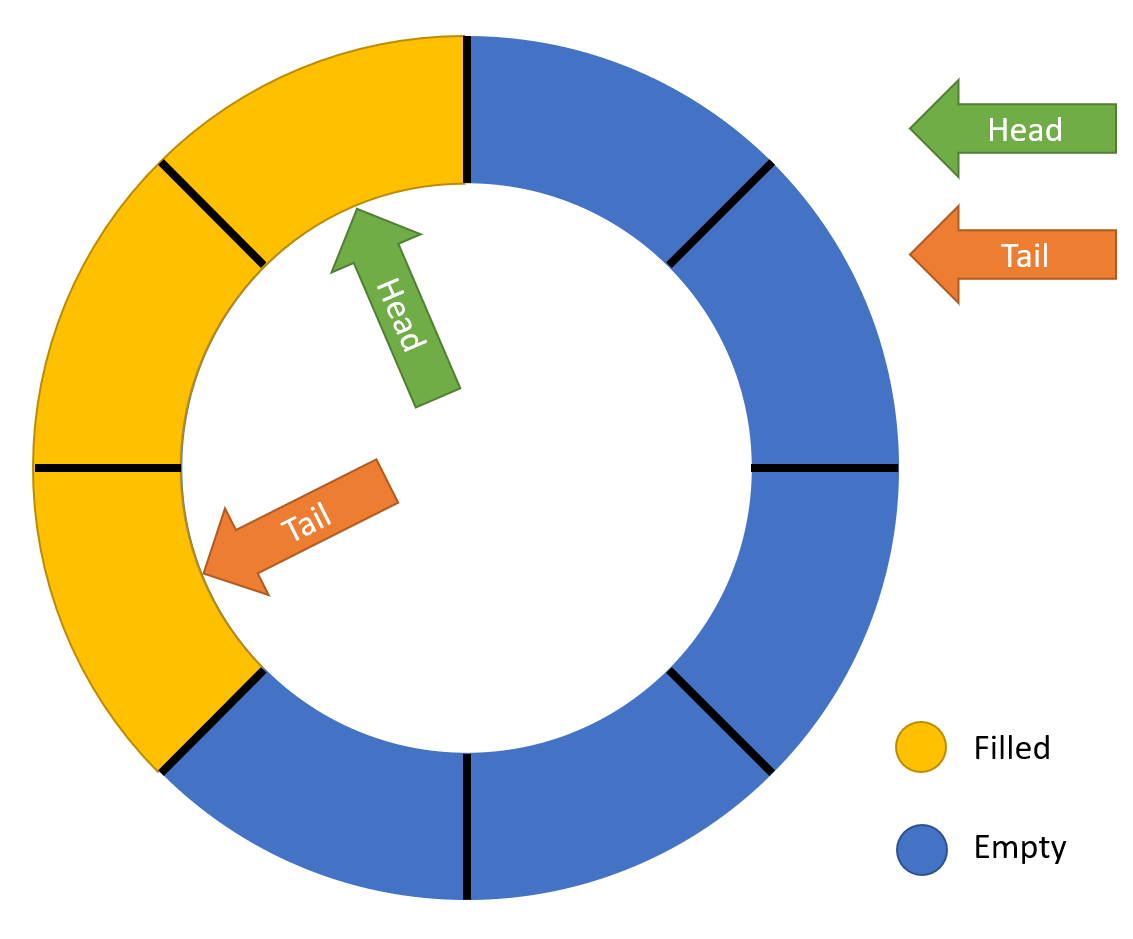
\includegraphics[scale=0.2]{Deque-Limited}
\caption{Deque from Array}
\label{fig:Img1}
\end{wrapfigure}
Die einfachste Möglichkeit eine Deque zu implementieren ist mithilfe eines Arrays. Dies wiederum hat Vor- und Nachteile. Ein Vorteil ist, dass der Speicherbereich der Datenstruktur bekannt ist, sowie auch alle darin befindlichen Adressen. Das bedeutet, dass man die darin befindlichen Adressen berechnen kann, sofern der Pointer auf den Speicherbereich bekannt ist. Ein Nachteil ist, dass die maximale Länge der Datenstruktur hierbei fixiert ist, und diese ohne weiteres nicht vergrößert werden kann. Wie man hier im Beispiel (Abbildung.~\ref{fig:Img1}) sehen kann, ist das Array auf acht Objekte beschränkt. Zwar kann die Deque im Rahmen dieser acht Elemente dynamisch anwachsen, sind die acht Elemente jedoch erreicht, ist die Warteschlange voll. Thematisch ist dieser Aufbau praktisch, um das Verhalten der Pointer innerhalb der Datenstruktur genauer betrachten zu können.  \newline
Sofern keine Objekte in der Deque gespeichert sind, zeigen Head- und Tail-Pointer auf „NULL“, woraus geschlussfolgert werden kann, dass die Datenstruktur leer sein muss. Dies gilt unabhängig davon, was tatsächlich in dem Speicherbereich selbst steht. Innerhalb der einzelnen Adressen haben die Daten einen undefinierten Zustand und sind somit be- bzw. überschreibbar. Mit dem Einfügen des ersten Objektes in die Datenstruktur werden die Pointer definiert. Head- und Tail-Pointer zeigen somit auf den selben ort im Speicher, in welche das erste Objekt gelegt worden ist. Welche Position für das erste Objekt genutzt wird, ist grundlegend irrelevant, da man alle weitere Adressen berechnen kann.\newpage 
\begin{lstlisting}[language=C, frame=single, style=customc]
void deque_add_front(void* value, deque_t* myQue){
   
 if(myQue->front == -1) {
        myQue->front = myQue->back = 0;
        myQue->array[myQue->front] = value;
        return;
    }

    if(myQue->front + 1 % MAX == myQue->back) {
        printf("\nThe Deque is full!\n");
        return;
    }

    if((myQue->front + 1) % MAX){
        myQue->front++;
        myQue->array[myQue->front] = value;
    }   else {
        myQue->front = 0;
        myQue->array[myQue->front] = value;
    }

    return;
}
\end{lstlisting}
Bei der hier beschriebenen Implementation wird das erste Objekt auf die nullte Position in das Array gelegt. Diese Adresse ist bekannt, da sie der Adresse auf dem Speicherbereich entspricht. Aufgrund dessen, dass die maximale Länge der Deque ebenso bekannt ist, ist dadurch auch die letzte Speicheradresse berechenbar. Versucht man nun, ein weiteres Objekt in die Warteschlange einzufügen, so wird der entsprechende Head-Pointer, für ein Einfügen am Head, bzw. der Tail-Pointer, für ein Einfügen am Tail, um eine Position verschoben. Hierbei müssen mehrere Probleme abgefangen werden. Zu Beginn wird überprüft, ob der potentiell verschobene Pointer dem anderen Pointer entspricht, also ob der Head-Pointer nach dem Verschieben auf den Tail-Pointer zeigen würde. Ist dem der fall ist die Deque an dieser stelle voll und es kann kein weiteres Objekt in die Warteschlange eingefügt werden. Wenn dem nicht so ist, wird überprüft, ob es zu einem Overflow kommt, also ob der Indexzähler des Arrays versucht, den reservierten Speicherbereich zu verlassen. Tritt dies ein, so wird der Index des Head-Pointers auf die letzte definierte Speicheradresse gelegt oder der Tail-Pointer auf die erste definierte Adresse. Im Anschluss wird nun das zu speichernde Objekt in die Speicherzelle gelegt und diese somit definiert. Versucht man jedoch, Objekte aus der Warteschlange zu entfernen, so müssen lediglich die Pointer auf diese Selle zurück verschoben werden, welche innerhalb des definierten Bereiches der Warteschlange liegt. Nachdem das Objekt gelesen wurde, muss somit kein tatsächlicher Löschvorgang ausgeführt werden und die Speicherbereiche werden als undefiniert betrachtet. Hierbei muss wieder beachtet werden, dass wenn der Index über die Definierten Bereiche hinaus geht, der Pointer auf die Entsprechend andere Seite definiert werden muss. Falls es durch wiederholtes Entfernen zu dem Fall kommt, dass beide Pointer wieder auf ein Objekt zeigen und dieses entfernt wird, müssen auch die Pointer einen undefinierten Zustand annehmen, was wieder signalisiert, dass die Deque leer ist.
Solange sich mindestens ein Element in der Warteschlange befindet, kann man durch wiederholtes Hinzufügen, bzw. Entfernen neuer Objekte den definierten Speicherbereich kreisförmig durch das Array bewegen, was in Abbildung~\ref{fig:Img1} verdeutlicht wurde. Dieses Verhalten jedoch ist einzigartig bei Deques mit statischer Größe.

\subsection{Deque mit dynamischer Länge}
Komplexer jedoch sind Deques welche dynamisch in der Länge anwachsen bzw. schrumpfen können. Hierbei wurden zwei verschiedene Herangehensweisen implementiert. Die Aspekte, mit welchen man dieses Kategorisieren kann, sind zum einem Speicheroptimierung und zum anderen Zugriffsgeschwindigkeit. 
\subsubsection{Deque - mit Double-Linked-List} 
\begin{wrapfigure}{l}{0.5\textwidth}
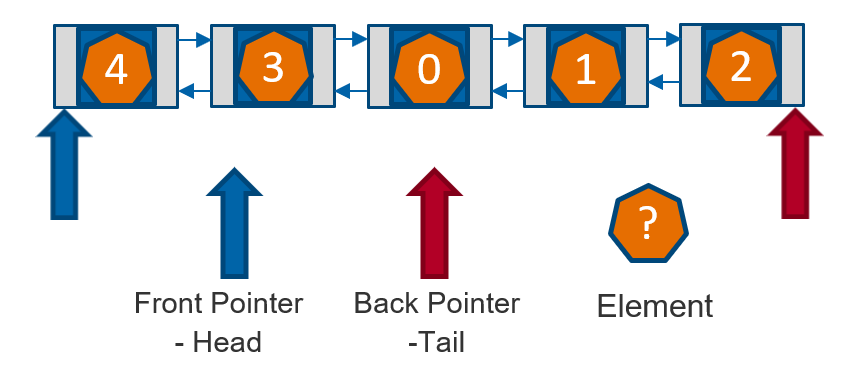
\includegraphics[scale=0.35]{Deque-LinkedList}
\caption{Deque from Double-Linked-List}
\label{fig:Img2}
\end{wrapfigure}
Implementiert man eine Deque mithilfe einer Double-Linked-List, ist die Grundfunktionalität, sich durch die Datenstruktur zu bewegen, bereits gegeben. Innerhalb einer Double-Linked-List kennt jedes Element das in der Warteschlange vor sich sowie hinter sich befindliche Element im Speicher. Hierbei ist wichtig, dass die vorherigen bzw. nachführenden Positionen mithilfe von Pointern gespeichert werden, was bewirkt, dass die Elemente nicht sequenziell im Speicher liegen. Dies wiederum hat Vor- und Nachteile. Ein Vorteil ist, dass beim Einfügen eines neuen Objektes in die Warteschlange ein neuer Bereich im Speicher für diesen alloziert wird. Somit kann die Warteschlange dynamisch anwachsen bzw. schrumpfen. Ein Nachteil jedoch ist, dass es nicht möglich ist die gespeicherten Elemente im Speicher zu zählen, ohne über die Elemente zu iterieren. Während man bei sequenziell im Speicher befindlichen Objekten die Endadresse des Speicherbereiches errechnen kann, ist hier jedes Element einzeln ein Definierter Speicherbereich, welcher auf einen anderen Zeigt. Zeigt einer der Pointer eines Elementes auf „NULL“, ist dies entsprechend ein Ende der Warteschlange. Hierbei müssen lediglich die beiden Elemente, worin jeweils ein NULL-Pointer gespeichert ist, gespeichert werden und man kann die Warteschlange von vorn bzw. hinten aufrufen. 
\begin{lstlisting}[language=C, frame=single, style=customc]
typedef struct DequeItem{
    struct DequeItem* previous;
    void* data;
    struct DequeItem* next;
} DequeItem_t;

typedef struct LinkedDeque{
    DequeItem_t* head;
    DequeItem_t* tail;
    int elementCount;
} LinkedDeque_t;
\end{lstlisting}
In der hier zu findenden Implementation werden zwei Structs verwendet. Zum Einem das Struct „DequeItem“, welches, wenn man eine Variable daraus erzeugt, in der Lage ist, die Daten, die man speichern möchte und zwei Pointer, welche auf andere Elemente dieses Typen zeigen, entgegenzunehmen. Dies spiegelt eines der blauen Elemente wider, wie es in der Abbildung~\ref{fig:Img2} zu sehen ist. Während „DequeItem“ die Double-Linked-List formt, werden in „LinkedDeque“ die beiden Enden der Datenstruktur gespeichert und die Elemente in der Deque gezählt. Somit wird für weitere Interaktion mit der Deque nur noch das „LinkedDeque“ item benötigt, da dieses sowohl den Head als auch den Tail beinhaltet. Erstellt man nun eine Deque, zeigen zu Beginn sowohl Head- als auch Tail-Pointer auf „NULL“ und die Variable des Element-Counters wird auf 0 gesetzt. Somit ist erkennbar, dass die Deque leer ist. 
\begin{lstlisting}[language=C, frame=single, style=customc]
void Deque_add_front(LinkedDeque_t* deque, void* item) {
    DequeItem_t* newHead = malloc(sizeof(DequeItem_t));
    newHead->data = item;
    newHead->next = deque->head;
    newHead->previous = NULL;
    if(deque->head == NULL) {
       deque->head = newHead; 
       deque->tail = newHead;
       deque->elementCount++;
    }
    else{
        deque->head->previous = newHead;
        deque->head = newHead;
        deque->elementCount++;
    }
}
\end{lstlisting}
Fügt man nun ein neues Objekt am Head ein wird ein „DequeItem“ erzeugt. Im Anschluss daran werden die Daten, welche in der Warteschlange gespeichert werden sollen, in dieses gelegt. Zudem wird der alte Head der Warteschlange benötigt und überprüft, ob dieser auf „NULL“ zeigt. Ist dem der Fall, so ist die Deque leer und es wird das neu erzeugte „DequeItem“ sowohl als Head als auch als Tail eingetragen und der Element counter um eins erhöht. Ist dem nicht der Fall, so muss lediglich in den alten Head der neue Head als vorangehendes Objekt eingetragen werden und der eben generierte Head in der „LinkedDeque“ als neuer Head gespeichert werden. Wenn dies geschehen ist, wird auch hier der Element counter um eins erhöht und es wurde erfolgreich der Deque ein Objekt am Head angefügt. Analog würde dies genau so mit dem Anfügen eines Objektes am Tail geschehen. Falls man Elemente lädt, wird entsprechend das Head- oder Tail-Objekt geladen. Darin befinden sich die zu ladenden Daten sowie die Adresse des folgenden Objektes, was als neuer Head bzw. Tail angenommen wird. Somit ist bei dieser Implementation der gesamte Speicher, welcher erzeugt wird, auch genutzt. Jedoch ist der Allokations-Prozess relativ langsam und wiederholt sich für das Einfügen jedes Objektes.

Im Gegensatz dazu wäre es effektiver, für mehrere einzufügende Datensätze nur wenige Speicher-Allokationsprozesse zu benötigen.
\subsubsection{Deque - mit Blocks}
\begin{figure}
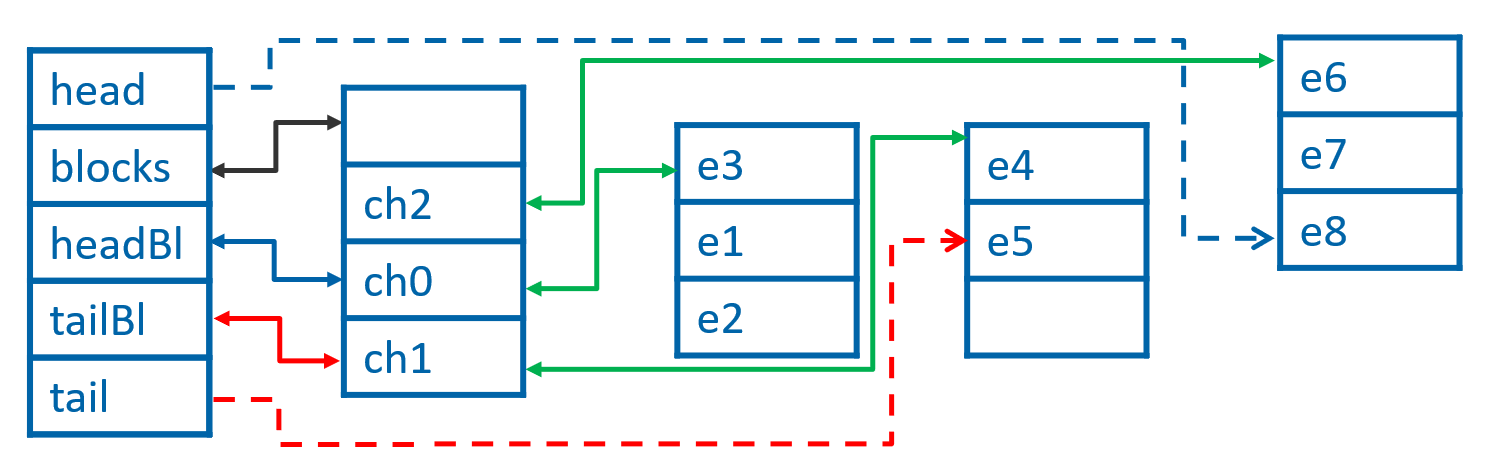
\includegraphics[scale=0.38]{deque-dyn}
\caption{Deque aus Blöcken}
\label{fig:Img3}
\end{figure}

Der Grundgedanke hinter der Double-Ended-Queue bestehend aus Blöcken ist, dass man sich Allokations-Zeit spart. Diese Ersparnis kommt zu Stande, indem man durch einen Allokations-Prozess Platz für mehrere zu speichernde Objekte schafft. Diese „Blöcke“, in denen man dann mehrere Objekte speichern kann, müssen jedoch auch individuell gespeichert werden, damit sie kontinuierlich adressierbar bleiben. An dieser Stelle ist zu beachten, dass die bisher einfache Implementierung der Head- und Tail-Pointer an Komplexität zunimmt. Hierbei kann der Fall auftreten, dass innerhalb eines Blocks weder Head- noch Tail-Pointer zu finden sind. Auch ist es nicht verpflichtend, dass Head- oder Tail-Pointer überhaupt im selben Block sind, da mit ansteigender Länge der Deque diese zunehmend auseinanderrücken. Somit werden hierbei zwei neue Variablen eingeführt, welche immer auf den Block zeigen, in dem sich der entsprechende Head- oder Tail-Pointer befindet. Der Vorteil dieser Implementation ist zwar der Zuwachs an Zugriffs und Speicher-Geschwindigkeit, jedoch kostet dies Speichereffektivität und kann zu sehr leeren, jedoch reservierten, Bereichen im Speicher führen.
Ein schematischer Aufbau dieser Implementation ist in Abbildung~\ref{fig:Img3} zu sehen. Erzeugt man nun eine neue Warteschlange, so muss zu Beginn erst eine Karte mit einer festgelegten Länge definiert werden. Zudem wird der Element counter hier wieder auf null gesetzt, da die Warteschlange nach dem Erzeugen noch keine Elemente hält. 
\begin{lstlisting}[language=C, frame=single, style=customc]
void deque_add_front(ctrItems_t* deque, void* item) {
    if(deque->elementCounter == 0) {
        deque->map[deque->mapLenght/2] = malloc(sizeof(void*) * BLOCKSIZE);
        deque->headBlockIndex = deque->mapLenght/2;
        deque->tailBlockIndex = deque->mapLenght/2;
        deque->headIndex = BLOCKSIZE/2;
        deque->tailIndex = BLOCKSIZE/2;
        deque->map[deque->headBlockIndex][deque->headIndex] = item;
        deque->elementCounter++;
        return;
    }
    if(deque->headIndex == 0) {
        if(deque->headBlockIndex == 0) {
            resizeMapHead(deque);            
        }
        deque->headBlockIndex--;
        deque->map[deque->headBlockIndex] = malloc(sizeof(void*) * BLOCKSIZE);
        if(deque->map[deque->headBlockIndex] == NULL) {
            printf("Could not allocate a new Block\n");
            return;
        }
        deque->headIndex = BLOCKSIZE - 1;
    }
    else {deque->headIndex--;}
    deque->map[deque->headBlockIndex][deque->headIndex] = item;
    deque->elementCounter++;
}
\end{lstlisting}
Fügt man nun ein Element in die Warteschlang, am Head ein, so wird überprüft, ob diese bereits Objekte beinhaltet. Ist dem nicht der Fall, so muss zu Beginn ein Block erzeugt werden. Dieser wird in die (relative) Mitte der Karte gelegt, damit genügend Platz in beide Richtungen vorhanden ist, um die Datenstruktur wachsen zu lassen. Die Pointer auf Head und Tail werden gesetzt, ebenso müssen die Pointer auf den Block, in ddem diese sich befinden, definiert werden. Zuletzt wird das zu speichernde Element in den Block gelegt und somit der Speicher definiert.\newline

Wiederholt man dies nun und fügt weitere Objekte ein, werden sich die Pointer innerhalb eines solchen Blocks so verhalten, wie man es schon bei der statischen Deque beobachtet hat. Verlässt jedoch einer der Pointer den definierten Index-Bereich des Blocks, so wird nicht wie bei der statischen Implementation der Pointer an das andere Ende des definierten Bereiches gelegt, sondern ein neuer Block erzeugt. Mit Erzeugen eines neuen Blocks muss in diesem Beispiel dementsprechend auch der Head-Pointer in diesen gelegt werden, was durch den „HeadBlock“ Pointer signalisiert wird. Dies kann nun wiederholt werden, bis die Karte an einer Stelle überläuft und der Headblock- bzw. Tailblock-Pointer den definierten Speicherbereich der Karte verlässt. Wenn dies der Fall ist, muss überprüft werden, ob die Karte voll ist, oder ob nur ein kleiner Teil des Speichers tatsächlich belegt wurde. 
\begin{wrapfigure}{l}{0.475\textwidth}
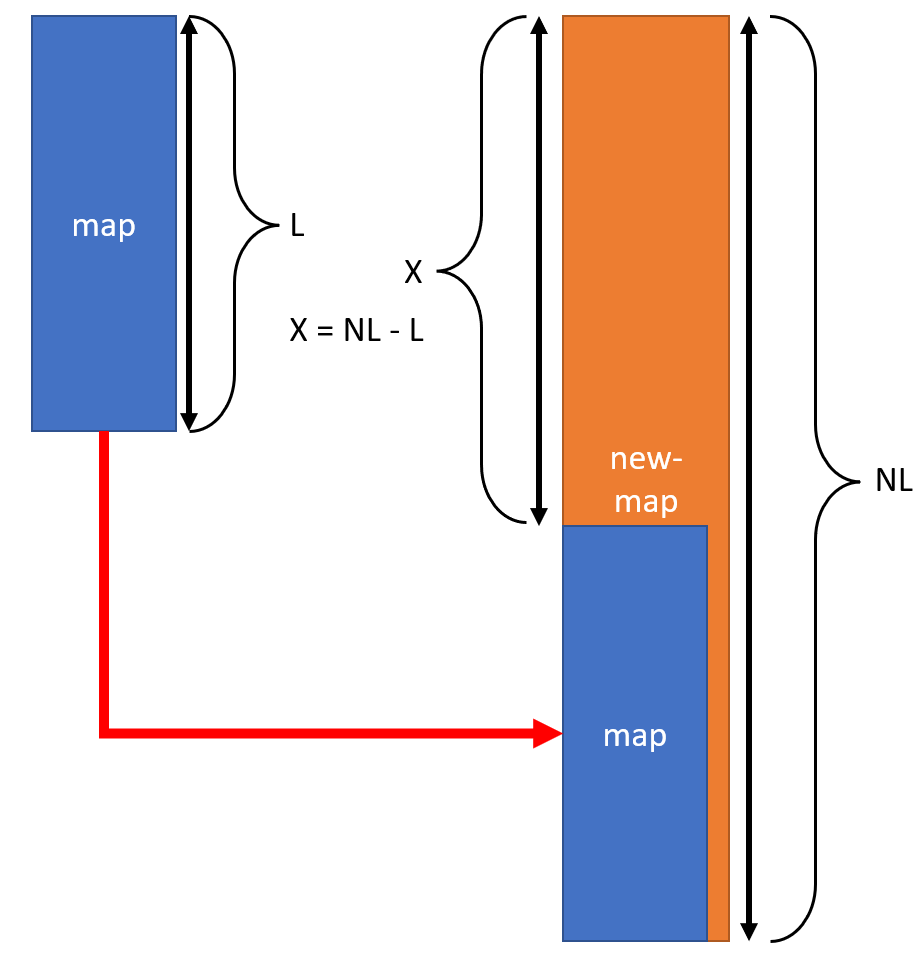
\includegraphics[scale=0.3]{MapAlloc}
\caption{Deque map positioning problem}
\label{fig:Img4}
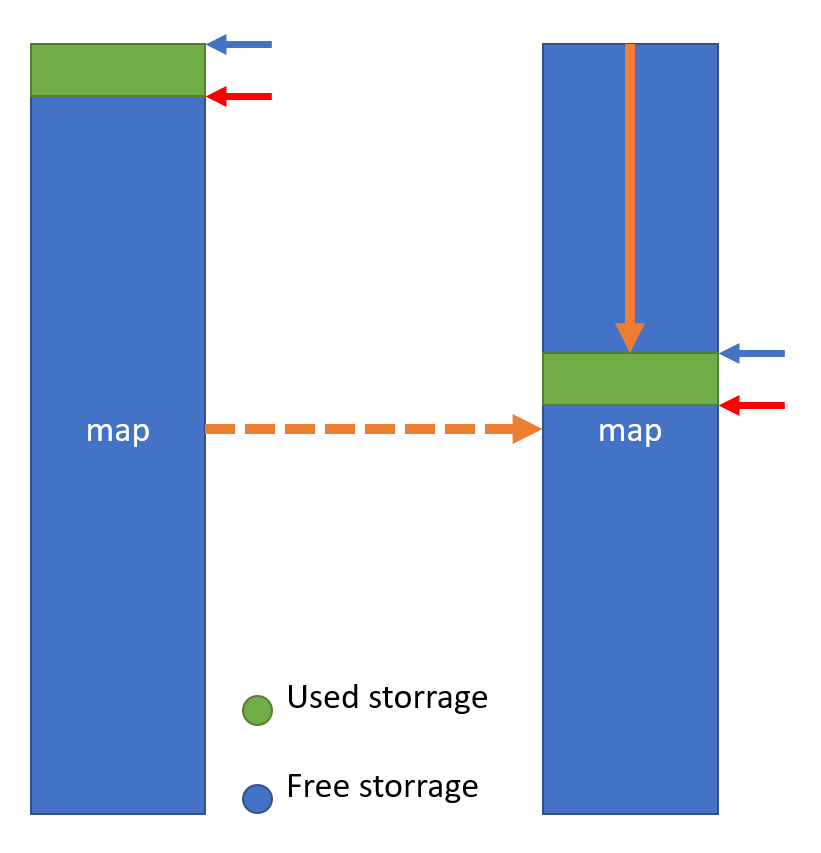
\includegraphics[scale=0.325]{MoveMap}
\caption{Deque einseitiger Überlauf}
\label{fig:Img5}
\end{wrapfigure}
Im Fall, dass die Karte tatsächlich voll ist und einseitig überläuft, wird eine neue Karte erstellt. Die neue Karte ist in dieser Implementation doppelt so groß wie die alte Karte. Als nächstes muss berechnet werden, wo die alte Karte in die neue gelegt werden muss. Hierzu ist zu beachten, an welcher Stelle der Überlauf stattgefunden hat. Ist dies am Head passiert, so muss der erstellte freie Speicherbereich vor der alten Karte sein. Betrachtet man nun die Abbildung~\ref{fig:Img4}, so wird eindeutig, dass man die alte Karte um X verschoben in die neue legen muss. Hierbei berechnet sich X einfach aus der Länge der neuen Karte (NL) minus die Länge der alten Karte (L). Der dadurch berechnete Index ist somit der Versatz, um welchen die alte Karte mit Hilfe von „memcpy“ in die neue kopiert werden muss. 
Falls der Überlauf am Tail stattfindet, muss hierbei die alte Karte lediglich in die neue gelegt werden, da diese kürzer ist als die neue und somit der freie Speicher nach der alten Karte übrigbleibt. \newline
An dieser Stelle jedoch abzufangen ist ein Überlauf der Karte, während die Warteschlange selbst im Verhältnis kaum Elemente beinhaltet. Somit der genutzte Speicher also nahezu leer ist. Dieses Verhalten tritt auf, wenn innerhalb der Deque mindestens ein Element befindlich ist und wiederholt, z.B. am Head Objekte angehängt werden, welche im Anschluss am Tail entfernt werden. In der statischen Deque würde sich hierbei der definierte Bereich des Speichers im Kreis bewegen. In dieser Implementation würde aufgrund dessen wiederholt in eine Richtung neuer Speicher reserviert werden, während die Warteschlange selbst nur wenige Objekte beinhaltet.
Somit muss beim Versuch, die Karte zu vergrößern zuerst überprüft werden, wie viele Blöcke tatsächlich Daten beinhalten. Wenn die Anzahl dieser unter einem Schwellenwert liegt, in dieser Implementation 30\%, muss ein Teil der freien Speicherblöcke vor die belegten geschoben werden. Dafür muss die Mitte der Karte und damit die zu bewegende Distanz des definierten Speichers berechnet werden. Abhängig davon, an welcher Seite der Überlauf stattgefunden hat, muss der Definierte Speicher so gelegt werden, dass entweder der Head oder der Tail in der Mitte der Karte ist. Im Anschluss davon müssen die HeadBlock- bzw. Tailblock- Pointer wieder angepasst werden.  
\begin{lstlisting}[language=C, frame=single, style=customc]
    if(1.0*currentFill/deque->mapLenght < 0.3) {
        int centerMap = deque->mapLenght/2;
        int distanceToMove = centerMap - deque->headBlockIndex;
        memmove(&(deque->map[centerMap]), &(deque->map[deque->headBlockIndex]), (currentFill*sizeof(void*)) );
        deque->headBlockIndex = deque->headBlockIndex + distanceToMove;
        deque->tailBlockIndex = deque->tailBlockIndex + distanceToMove;
        return;
    }
\end{lstlisting}
Nach dem Verschieben des definierten Speichers, kann die Deque somit weiterverwendet werden. Das wichtige dabei ist: nach Abschluss dieser Funktion ist die Größe der Karte konstant geblieben und die Blöcke selbst sowie die Head- bzw. Tail-Pointer wurden auch nicht verschoben. 
\section{Benchmarks}
Alle drei Implementationen, welche in 3. Aufbau der Deque benannt wurden, sind mit unterschiedlichen Ansprüchen belegt. Konzeptionell funktionieren diese Warteschlangen alle gleich, dennoch kann man Vermutungen zu ihrer Performance aufstellen. Da die Implementation mit einem Array eine Fixierte Größe besitzt, müsste diese alle anderen Implementationen im Zugriff und Speichergeschwindigkeit übertreffen. Kurz darauf müsste die dynamische Implementation mit Blöcken einzusortieren sein. Die Implementation mit einer Double-Linked-List müsste hierbei die langsamsten Zugriffe und Speichervorgänge aufweisen.
Im Rahmen dieser Seminararbeit wurden alle drei Umsetzungskonzepte vollständig implementiert und verglichen. Mit diesen wurden im Anschluss darauf drei versuche erstellt, um ihre Funktionalität und Performance zu überprüfen und die voranstehenden Behauptungen zu bestätigen. 
\subsection{Versuch „Einfügen mit Anfangswerten“}
In diesem Versuch wurde für alle drei Datenstrukturen untereinander verglichen, wie sie sich verhalten, wenn sich bereits Daten in der Warteschlange befinden. Dabei wurden 10 Millionen Einträge jeweils in sie gelegt, bevor der Test gestartet wurde und während des Testes 50 Millionen weitere. Hierbei wurden die vorher benannten Erwartungen an diese gestellt. Die Ergebnisse davon sind auf Seite~\pageref{fig:Array10-50},~\pageref{fig:Linked10-50} und~\pageref{fig:Block10-50} zu finden und bestätigen damit die gestellten Vermutungen.
Betrachtet man nun die einzelnen Implementationen ist zu sehen, dass diese ein annährend lineares Verhalten beim Einfügen der Daten in die Datenstruktur aufweisen. Dies bedeutet, dass alle Einfügevorgänge hierbei in etwa die gleiche Zeit in Anspruch nehmen. Dies ist im zweiten Diagramm auf den jeweiligen Seiten aufgeführt. Die dort ersichtlichen Abweichungen sind damit zu erklären, dass nicht gewährleistet ist, dass der Benchmark-Prozess während der gesamten Ausführungszeit ohne Unterbrechung die CPU zugewiesen bekommen hat. Zudem kann bei der Implementation mit der Double-Linked-List und jener mit den Blöcken noch in Frage gestellt werden, ob die malloc Aufrufe alle eine gleiche Geschwindigkeit aufweisen, um Speicher zu allozieren. Um dem entgegenzuwirken, wurde der Test mit entsprechend vielen Daten vollzogen, um einen sinnvollen Durchschnitt bilden zu können.
\subsection{Versuch „Einfügen ohne Anfangswärte“}
In diesem Benchmark wurde Versucht, das verhalten ein weiteres mal zu bestätigen, was auf den Seiten~\pageref{fig:Array0-60},~\pageref{fig:Linked0-60} und~\pageref{fig:Block0-60} ersichtlich ist. Zudem wurde dieser Versuch gehalten, um zu sehen, ob es einen merklichen Unterschied macht, wenn die Warteschlange zu Beginn leer ist. Dies sollte bei der Implementation mit Blöcken zumindest theoretisch einen Unterschied machen, da diese mit ansteigender Länge zunehmend weniger Allocationsprozesse der Karte selbst durchführen muss. Dies ist jedoch in den Benchmarks nicht festzustellen. Es lässt sich daraus schließen, dass diese zunehmend langen malloc Prozesse einen insignifikanten Unterschied im Vergleich zur gewonnenen Performance bei der zur Implementation mit einer Double-Linked-List aufweist.  
\subsection{Versuch „Zugriff“}
Zuletzt wurde in diesem Versuch das Verhalten der Warteschlangen beobachtet, wenn aus ihr Elemente entfernt werden. Hierbei zu sehen ist, dass wie auch beim Einfügen der Elemente dies eine annährend lineares Verhalten aufweist. Auf dem ersten Graf auf Seite~\pageref{fig:Zugriff} ist zu sehen, dass die Zugriffszeit zwischen Block Implementierung und Array nahezu identisch ist. Es ist auch zu erkennen, dass die Deque aus der Double-Linked-List konsequent langsamer ist als die anderen beiden. Dies bestätigt wieder die vorangegangene Annahme. Somit lässt sich feststellen, dass die Deque aus Blöcken einen Großteil der Vorteile mit sich bringt, welche die des Arrays hat, und gleichzeitig die Dynamik der Double-Linked-List. Auch hier ist jedoch wieder die Zugriffszeit Abweichung welche schon vorher beim einfügen verzeichnet wurde zu sehen, was wieder mit der zugewiesenen zeit der CPU erklärt werden kann.
\section{Anwendung}
Die Illusion, dass Computer Prozesse gleichzeitig ausführen, ist ihrer Geschwindigkeit und Optimierung zu verdanken. Zudem werden Prozesse in Threads aufgeteilt, welche nacheinander oder durcheinander ausgeführt werden können. Diese dienen dazu, einen Prozessorkern nicht warten zu lassen. Zeit, in der ein Prozessor auf etwas wartet, ist verschwendete Rechenkapazität und der Gedanke hierbei ist es, ihn schon an anderen Threads arbeiten zu lassen, während z.B. auf antworten von Webseiten gewartet wird. So werden bei Parallelrechnern verschiedene scheduling Strategien verwendet, wie z.B. das Work-Stealing.
\subsection{Work-Stealing}
\label{WorkStealing}
Work-Stealing ist eine Multithreading-Strategie, wie sie in Parallelrechnern Anwendung findet. Hierbei haben verschiedene Prozessoren oder Kerne jeweils Warteschlangen, worin ihre Arbeitsaufträge (Threads) auf eine Bearbeitung warten. Während mit dem Start eines Programms nur eine gewisse Anzahl an Threads generiert werden, und versucht wird, diese so sinnvoll wie möglich auf die Prozessoren aufzuteilen, können einzelne Threads bei ihrem sequenziellen Ausführen auch neue generieren. Diese hier neu generierten Threads werden dann standardmäßig an das Ende der eigenen Warteschlange des Prozessors angehängt. Beim Ausführen eines Threads kann es jedoch auch dazu kommen, dass der aktuelle Thread pausiert werden muss. In diesem Fall würde der Prozessor versuchen, einen anderen Thread aus dem Head seiner Warteschlange zu laden. Alternativ kann ein Thread beendet sein, was zu einem gleichen Verhalten wie beim Pausieren führt. Kommt es nun zu dem Fall, dass ein Prozessor, oder auch Worker genannt, versucht auf seine Warteschlange zuzugreifen, diese jedoch leer ist, kann dieser anstelle seiner eigenen Warteschlange proaktiv (im Vergleich zum Work-Sharing \cite[721]{blumofe1999scheduling}) auf die Warteschlange eines andern Prozessors zugreifen. Somit wird der Prozessor zu einem Stealer. Da es jedoch ineffektiv ist, den Prozessor-Cache für einzelne Threads zu verwerfen, und sequenzielle Threads dies meist auch nicht benötigen, würde ein Eingreifen des Stealers auf die folgenden Aufträge des Workes hierbei eine relativ große Störung erzeugen. Dies kann umgangen werden, indem ein Stealer nicht versucht, sich Threads vom Head der Warteschlange eines Workers zu nehmen, sondern stattdessen auf den Tail zugreift. Hierbei kommt das Verhalten einer Double-Ended-Queue zum Einsatz. Als Letztes kann ein Thread noch einen anderen Thread aktivieren, welche diesen aus der Warteschlange des Prozessors heraus an den Kopf der Deque setzt, aber den aktuellen Thread erst zu ende bearbeitet.
Stiehlt ein Prozessor einem anderen einen seiner Threads, so können diese nun parallel nebeneinander ausgeführt werden, was die Ausführgeschwindigkeit des Prozesses erhöht und die Prozessoren/Kerne am Arbeiten hält. Beim Versuch einen Thread von einem anderen Prozessor zu stehlen, wird eine Warteschlange eines anderen Prozessors zufällig gewählt. Falls diese auch leer ist und somit zu einem Stealer geworden ist, wird dies so oft wiederholt, bis eine Warteschlange gefunden wurde, welche Threads beinhaltet. 

\section{Fazit}
Zugriff und Zugriffszeit auf Head und Tail. Der treibende Gedanke hinter der Datenstruktur Double-Ended-Queue. Wie in den Benchmarks dieser Arbeit bereits erläutert, sind die drei Implementationen, welche hier vorbereitet wurden, sehr unterschiedlich und doch gleich. Der Anspruch an eine Double-Ended-Queue ist es, eine Zugriffszeit O(1) nicht nur auf den Head einer Warteschlange zu gewährleisten, wie dies schon von normalen Warteschlangen getan wird, sondern auch auf den Tail. Wie im Kapitel der Benchmarks bereits belegt, weisen die Implementationen, welche im Rahmen dieser Arbeit entstanden sind, diesen Aspekt auf. Dennoch sind sie unterschiedlich. Dabei wurden drei verschiedene Möglichkeiten, eine Deque aufzubauen, vorgestellt. Baut man diese mithilfe eines Arrays, so ist sie im Vergleich mit den anderen Implementationen die schnellste, um auf die Daten zuzugreifen. Dies geschieht jedoch auf Kosten der Fähigkeit, dynamisch anwachsen zu können. Somit hat diese Implementation eine statische Länge und kann volllaufen. Zudem verbraucht sie im Vergleich zu den anderen Implementationen viel Speicher, welcher evtl. nicht benötigt wird, da dieser mit Erstellen der Deque bereits reserviert werden muss.Ist die Warteschlange somit nahezu leer, verbraucht die Datenstruktur im Speicher genauso viel platz wie als würde sie ihre maximale Kapazität erreicht haben. Um diesem Verhalten entgegenzuwirken und dennoch die Funktionalitäten der etablierten Funktionen zu wahren, wurde als ein weiterer Ansatz eine Double-Ended-Que aus einer Double-Linked-List implementiert. Diese hat den Vorteil, dass sie zum Einem dynamisch anwachsen und somit nicht volllaufen kann. Zudem wird von dieser Implementation nur der Speicher belegt, welcher tatsächlich von der Warteschlange benötigt wird. Vergleicht man jedoch die Performance dieser Implementation mit der des Arrays, wird sehr schnell klar, dass diese im vergleich langsam ist. Um die Performanten Zugriffs- und Speicherzeiten jedoch zu wahren, ist als letztes eine Implementation entstanden, welche den Mittelweg zwischen Speichereffizienz und Performance bietet. Im direkten vergleich mit den anderen jeweilig ein wenig schlechter, bietet die Implementation aus Blöcken jedoch eine Zugriffs- und Speicherzeit fast wie die des Arrays, mit der Fähigkeit dynamisch anwachsen zu können. Hierbei wird beim Einfügen direkt für weitere Einfügeprozesse Speicher reserviert. Weiterer Speicher wird jedoch erst reserviert, wenn der aktuelle Speicher in jeweils eine Richtung voll ist. Da diese Implementation somit performant, dynamisch und relativ Speicherfreundlich ist, ist anzunehmen, dass diese Implementation, die am weitesten verbreitete bzw. verwendete ist. 
\newpage
\section{Tabellen}
\begin{figure}[H]
\label{fig:Array10-50}
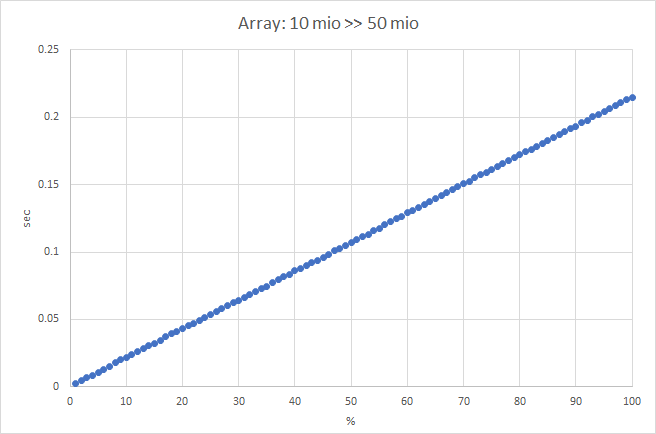
\includegraphics[scale=0.9]{Array10-50}
\begin{center}
\includegraphics[scale=1]{Array10-50-Time}
\end{center}
\end{figure}

\begin{figure}[H]
\label{fig:Array0-60}
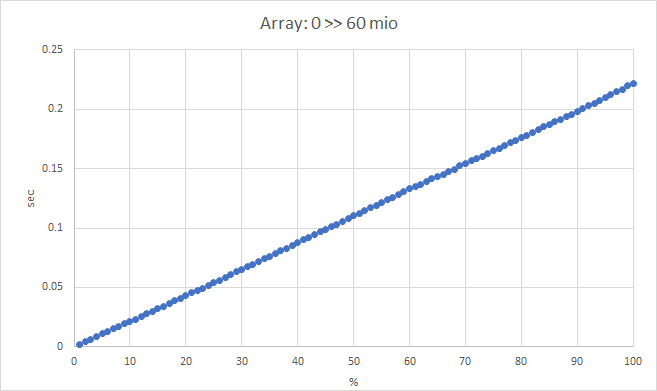
\includegraphics[scale=0.9]{Array0-60}
\begin{center}
\includegraphics[scale=1]{Array0-60-Time}
\end{center}
\end{figure}

\begin{figure}[H]
\label{fig:Linked10-50}
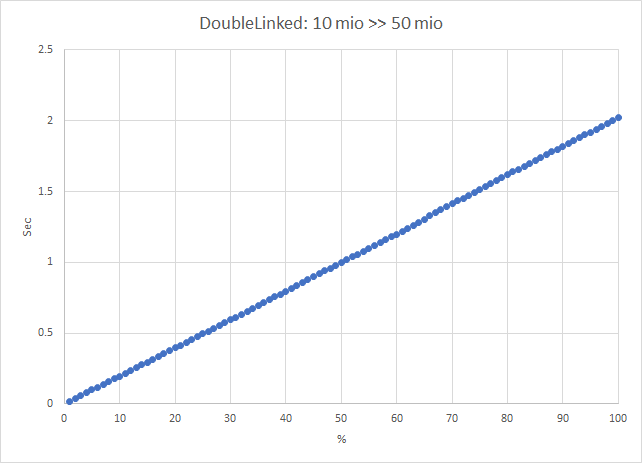
\includegraphics[scale=0.9]{Linked10-50}
\begin{center}
\includegraphics[scale=1]{Linked10-50-Time}
\end{center}
\end{figure}

\begin{figure}[H]
\label{fig:Linked0-60}
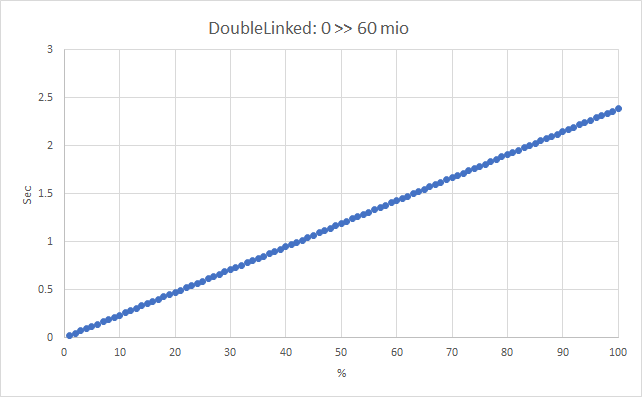
\includegraphics[scale=0.9]{Linked0-60}
\begin{center}
\includegraphics[scale=1]{Linked0-60-Time}
\end{center}
\end{figure}

\begin{figure}[H]
\label{fig:Block10-50}
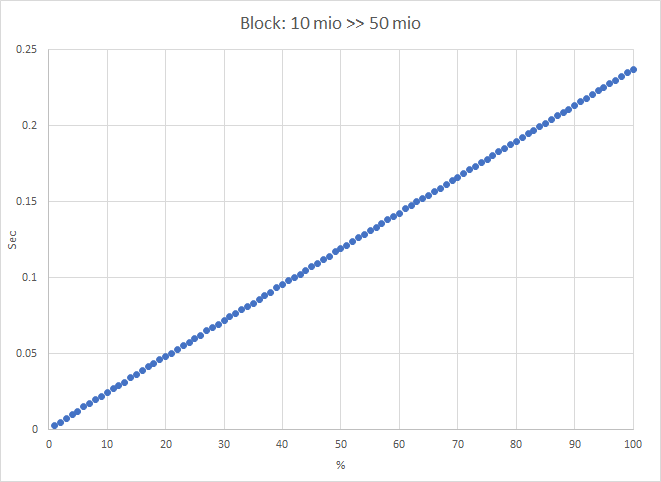
\includegraphics[scale=0.9]{Block10-50}
\begin{center}
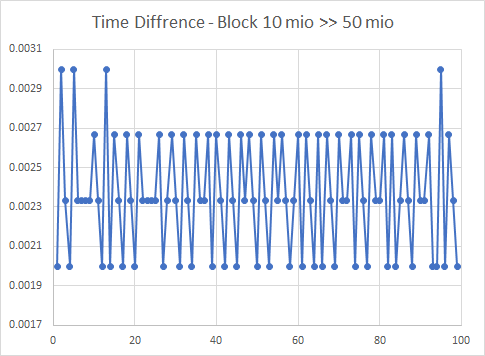
\includegraphics[scale=1]{Block10-50-Time}
\end{center}
\end{figure}

\begin{figure}[H]
\label{fig:Block0-60}
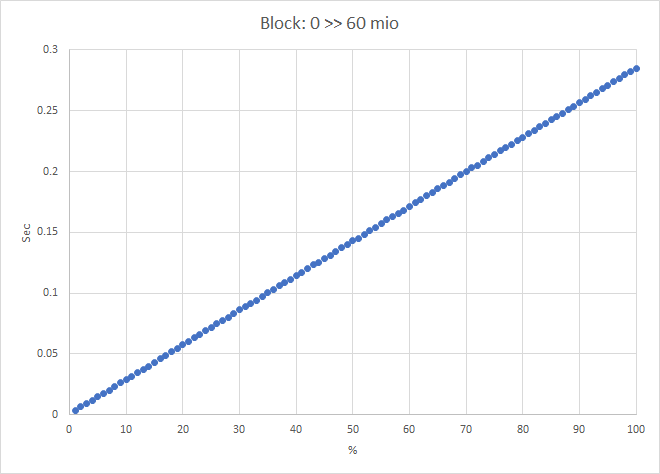
\includegraphics[scale=0.9]{Block0-60}
\begin{center}
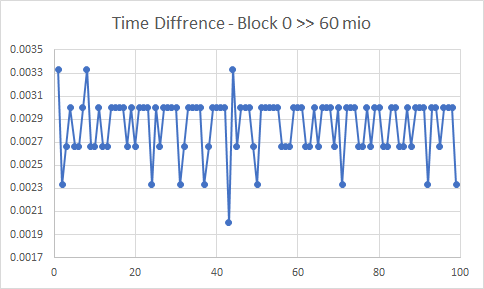
\includegraphics[scale=1]{Block0-60-Time}
\end{center}
\end{figure}

\begin{figure}[H]
\label{fig:Zugriff}
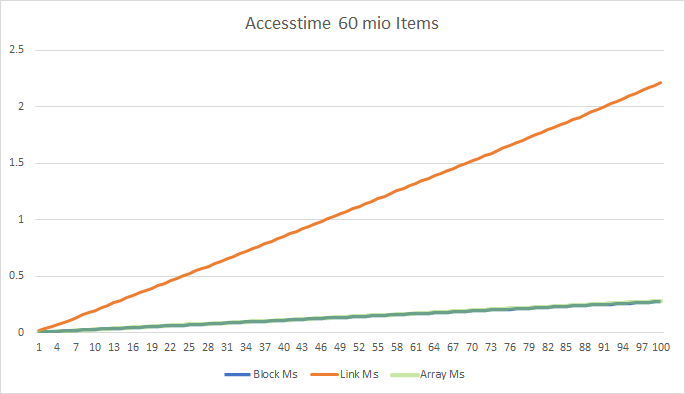
\includegraphics[scale=0.9]{Zugriff}

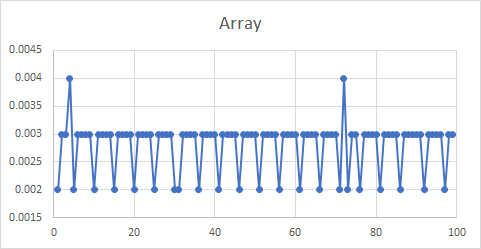
\includegraphics[scale=0.635]{ArrayVarriation}
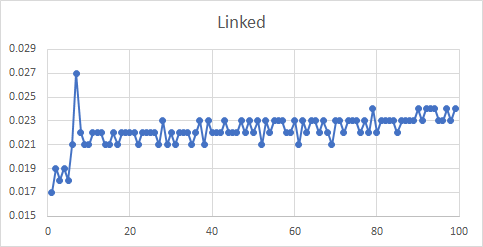
\includegraphics[scale=0.635]{LinkVarriation}
\begin{center}
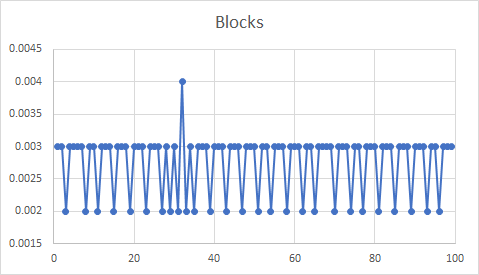
\includegraphics[scale=0.635]{BlockVarriation}
\end{center}
\end{figure}


\newpage
\bibliographystyle{alpha}
\bibliography{bibo}



\newpage
\section{Eidesstattliche Erklärung}
Ich versichere, dass ich diese Arbeit selbstständig verfasst und keine anderen Hilfsmittel als
die angegebenen benutzt habe. Die Stellen der Arbeit, die anderen Werken dem Wortlaut oder
dem Sinn nach entnommen sind, habe ich in jedem einzelnen Fall unter Angabe der Quelle
als Entlehnung kenntlich gemacht. Diese Versicherung bezieht sich auch auf die bildlichen
Darstellungen.\\ \\ \\ \\ \\ \\ \\
15.09.2021 \hfill Marco Naumann


\end{document}